\begin{frame}
\frametitle{What is (Big) Data?}
\vskip 1.0cm
\textit{From Wikipedia: \textcolor{isvblue}{qualitative or quantitative} variables for analysis}
    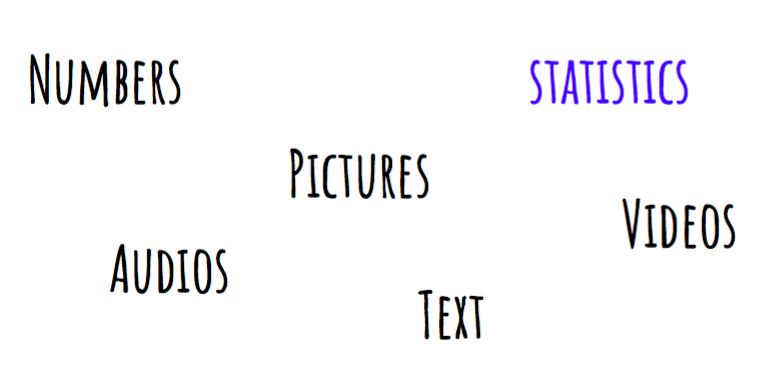
\includegraphics[width=1.0\textwidth]{./pictures/data-what.png}\\
\textcolor{isvblue}{The size of the data is a \textbf{spatiotemporal notion}!} 
\end{frame}

\begin{frame}
\frametitle{What do we do with (Big) Data?}
\vskip 0.8cm
Analyze (Big) Data to \textcolor{isvblue}{understand} and make some \textcolor{isvblue}{predictions} in:
\begin{itemize}
  \item \textcolor{isvblue}{Medicine}: to accelerate diagnosis and personnalize treatments  
  \item \textcolor{isvblue}{Government authorities}: to improve infrastructures and city operations (ex: Open Data platform by NYC)
  \item \textcolor{isvblue}{Social research}: to deepen understand social demography
  \item \textcolor{isvblue}{Marketing}: to understand customers and target strategies
  \item \textcolor{isvblue}{Journalism}: to investigate (Matt Caroll from Spotlight)
  \item (...) \textcolor{isvblue}{To innovate}
\end{itemize}
\end{frame}

\begin{frame}
\frametitle{Progress, Challenges, which Role to play?}
\vskip 0.8cm
    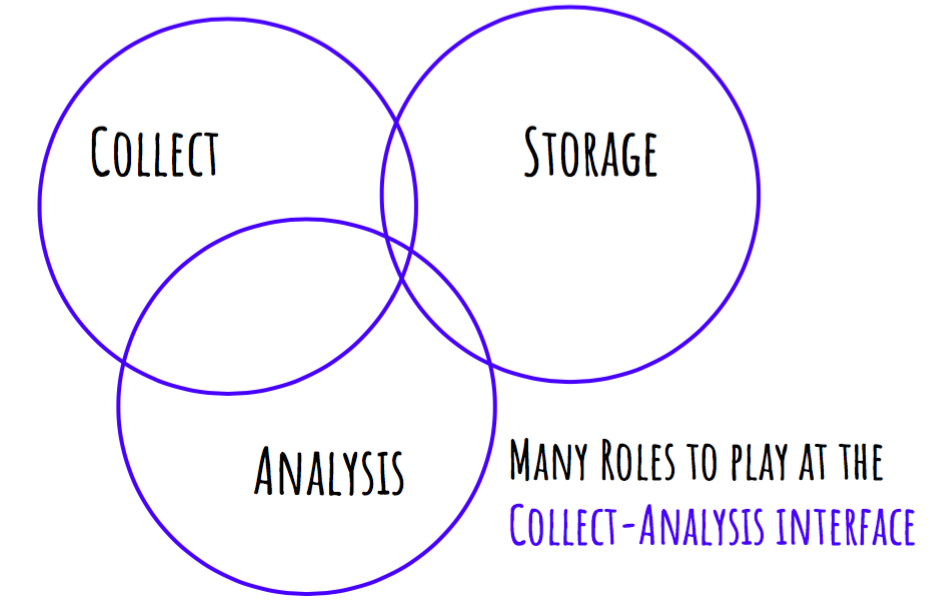
\includegraphics[width=1.0\textwidth]{./pictures/roles-in-data.png}\\
\end{frame}

\begin{frame}
\frametitle{(Big) Data Collect-Analysis interface}
\vskip 1.0cm
    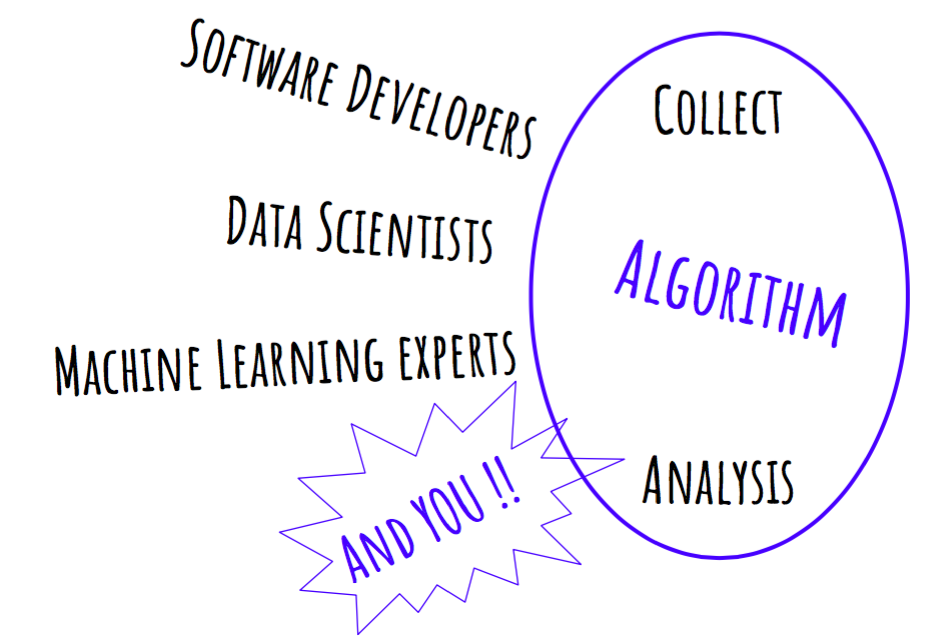
\includegraphics[width=1.0\textwidth]{./pictures/role-2.png}\\

\end{frame}

